\chapter{黑洞熵、全息原理與德西特空間}

\lectureoverview{我們將完成上一講開始的對應關係論證。高度激發的弦，其熵正比於質量；施瓦茲希爾德黑洞的熵則正比於面積。兩個公式之所以能夠連結，並非因為強引力黑洞等同於自由弦，而是因為緩慢調整弦耦合，讓兩種描述逐漸接合。面積定律自然導向全息原理；本講最後將介紹膨脹空間，以及下一講要探討其視界的德西特幾何。}

\section{回到計數問題}

長弦的計數還有一個問題尚未解決。如果把固定的總長度分配給數條弦，長度相同、性質全同的弦便不可區分。不過，它們在盒子中的位置仍屬於態的一部分；盒子的大小則選為大致符合相應單條長弦所佔據的區域。

\begin{classroomqa}
\audiencequestion{短弦彼此可以區分嗎？它們的位置要計入嗎？\lecturetimestamp{00:00:37}}
\lecturerresponse{性質全同的弦不可區分，但它們在盒子中的位置要計入。比較是在體積固定的條件下進行，所選體積與長弦所佔據的區域相當。}
\end{classroomqa}

這個問題釐清後，就可以說明我們的目標：整理出一小組方程式，藉此推得黑洞熵的標度關係。不需要計算積分或無窮級數。困難不在代數，而在於判斷哪些量可以比較，以及應該在論證的哪個階段進行比較。

\section{自然單位與普朗克面積}

令
\begin{equation}
c=\hbar=1,
\label{eq:l07-natural-units}
\end{equation}
但保留牛頓常數。首先可知，時間與長度具有相同的單位。由光子的關係式
\begin{equation}
E=\frac{\hbar c}{\lambda}
\end{equation}
以及質能關係式 \(E=mc^2\)，可得
\begin{equation}
[M]=L^{-1}.
\label{eq:l07-mass-dimension}
\end{equation}
因此，質量可以用長度的倒數表示。

\begin{figure}[htbp]
\centering
\includegraphics[width=0.62\textwidth]{lecture_07_figure_02.png}
\caption{量綱論證開頭採用的自然單位慣例。能量公式已補充於上方方程式中。}
\lectureframe{00:03:27.900}
\end{figure}

要判定 \(G_N\) 的單位，可把牛頓加速度公式僅用於量綱分析：
\begin{equation}
a\sim\frac{G_NM}{R^2}.
\end{equation}
由於 \(T\) 和 \(L\) 的單位相同，因此 \([a]=L/T^2=L^{-1}\)。再結合方程式~\eqref{eq:l07-mass-dimension}，可得
\begin{equation}
[G_N]=L^2.
\end{equation}
在這組單位下，牛頓常數具有面積的量綱。定義普朗克長度為
\begin{equation}
G_N=\ell_p^2,
\label{eq:l07-planck-area}
\end{equation}
便能立即看出 \(A/G_N=A/\ell_p^2\) 是無量綱的：它表示以普朗克面積為單位的面積。

\section{弦耦合與引力強度}

接著要用弦的語言描述引力。一個有用的圖像是交換過程：弦與自身交叉時，可能分裂後再重新接合。一個小的閉弦圈可以由一個物體發射，再由另一個物體吸收；若這個激發是引力子，該過程便傳遞引力。發射與吸收各帶有一個相互作用因子，因此交換強度含有 \(g_s^2\)。

耦合常數 \(g_s\) 是無量綱的。更精確地說，它是振幅層次的耦合；機率或反應率則從 \(g_s^2\) 階開始。\editorialnote{本講有時將 \(g_s\) 稱為機率，之後又更正為機率的平方根。微擾耦合屬於振幅層次。}由於 \(G_N\) 的量綱是面積，因此還需要一個長度尺度。基本弦長 \(\ell_s\)，也就是基本弦振動的尺度，正好提供這個尺度：
\begin{equation}
G_N\sim g_s^2\ell_s^2,
\qquad
\ell_p\sim g_s\ell_s.
\label{eq:l07-planck-string}
\end{equation}

\begin{figure}[htbp]
\centering
\includegraphics[width=0.72\textwidth]{lecture_07_figure_05.png}
\caption{黑板上的耦合關係：\(G_N=\ell_p^2\)與\(g_s^2\ell_s^2\sim\ell_p^2\)。}
\lectureframe{00:12:15.000}
\end{figure}

在弱耦合情況下，\(g_s\ll1\)，普朗克長度遠小於弦長。調低 \(g_s\)會減弱引力，同時維持基本弦尺度不變。\editorialnote{在有效四維理論中，緊緻化資料與數值慣例也會影響 \(G_N\)。在此標度論證中，這些因素都固定不變，並予以略去。}

\section{計數長弦}

熵反映的是描述一個態所需的基本選擇數目。把高度激發的弦近似成在正方格點陣上行走的路徑。每到一個頂點，下一段可朝四個方向之一延伸。把每次選擇說成四選一，或說成兩次二選一，只會改變一個數量級為一的常數；真正重要的是步數。

若 \(L\) 是弦的輪廓長度，而每一步長為 \(\ell_s\)，則需要
\begin{equation}
N=\frac{L}{\ell_s}
\end{equation}
步。路徑數呈指數成長，概略而言為 \(\Omega_N\sim q^N\)，其中 \(q\) 的量級為一，因此
\begin{equation}
S_{\mathrm{str}}=\log\Omega_N\sim N\sim\frac{L}{\ell_s}.
\label{eq:l07-string-entropy-length}
\end{equation}

\begin{figure}[htbp]
\centering
\includegraphics[width=0.68\textwidth]{lecture_07_figure_03.png}

\vspace{0.7em}
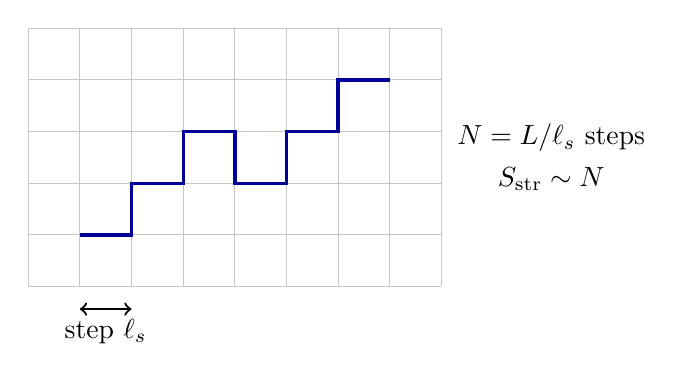
\begin{tikzpicture}[scale=0.82]
  \draw[step=0.8cm,gray!45,thin] (0,0) grid (6.4,4.0);
  \draw[very thick,blue!60!black]
    (0.8,0.8)--(1.6,0.8)--(1.6,1.6)--(2.4,1.6)--(2.4,2.4)--
    (3.2,2.4)--(3.2,1.6)--(4.0,1.6)--(4.0,2.4)--(4.8,2.4)--
    (4.8,3.2)--(5.6,3.2);
  \draw[<->,thick] (0.8,-0.35)--(1.6,-0.35);
  \node[below] at (1.2,-0.35) {step \(\ell_s\)};
  \node[align=center] at (8.1,2.0) {\(N=L/\ell_s\) steps\\[0.3em]\(S_{\mathrm{str}}\sim N\)};
\end{tikzpicture}
\caption{黑板上的格點模型，以及整理後的隨機漫步詮釋。決定選擇數目的，是弦的輪廓長度，而不是纏繞成團的球體直徑。}
\lectureframe{00:17:20.000}
\end{figure}

質量也可用相同的基本線段來計算。長度為 \(\ell_s\) 的線段，其質量尺度為
\begin{equation}
m_{\mathrm{seg}}\sim\frac{1}{\ell_s}.
\end{equation}

\begin{classroomqa}
\audiencequestion{基本線段的長度取為 \(\ell_s\) 嗎？\lecturetimestamp{00:18:56}}
\lecturerresponse{是。它的特徵長度是 \(\ell_s\)，因此在自然單位下，特徵質量是 \(1/\ell_s\)。}
\end{classroomqa}

把 \(L/\ell_s\) 段線段的質量加總，可得
\begin{equation}
M\sim\frac{L}{\ell_s}\frac{1}{\ell_s}
=\frac{L}{\ell_s^2},
\qquad
L\sim M\ell_s^2.
\label{eq:l07-string-mass}
\end{equation}
這個標度關係已將振盪弦的動能與位能概括在內；若進行詳細的統計力學計算，也會得到相同的依賴關係。代入方程式~\eqref{eq:l07-string-entropy-length}，便得到我們需要的弦熵公式：
\begin{equation}
S_{\mathrm{str}}\sim M\ell_s.
\label{eq:l07-string-entropy-mass}
\end{equation}

\begin{figure}[htbp]
\centering
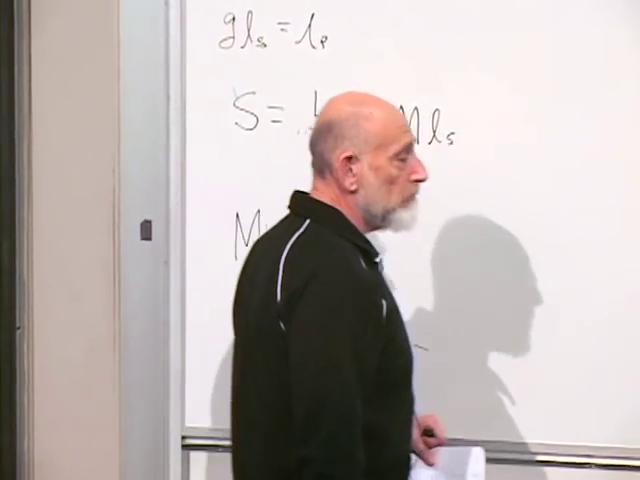
\includegraphics[width=0.66\textwidth]{lecture_07_figure_04.png}
\caption{比較前先整理弦這一側的關係：\(\ell_p\sim g_s\ell_s\)、\(S_{\mathrm{str}}\sim L/\ell_s\sim M\ell_s\)與\(M\sim L/\ell_s^2\)。}
\lectureframe{00:21:57.800}
\end{figure}

\section{為何自由弦還不是黑洞}

在引力這一側，精確的半經典公式是
\begin{equation}
S_{\mathrm{BH}}=\frac{A}{4G_N}.
\label{eq:l07-bh-exact}
\end{equation}

\begin{classroomqa}
\audiencequestion{分母中的數值係數應該是多少？\lecturetimestamp{00:23:28}}
\lecturerresponse{是四。對應關係論證可以得到標度關係，但過於粗略，無法確定這個精確因子。}
\end{classroomqa}

對四維施瓦茲希爾德黑洞而言，
\begin{equation}
R_s=2G_NM,
\qquad
A=4\pi R_s^2.
\end{equation}
依照本講的做法略去數值常數，
\begin{align}
S_{\mathrm{BH}}
&\sim\frac{A}{G_N}
\sim\frac{(G_NM)^2}{G_N} \\
&\sim M^2G_N
\sim M^2\ell_p^2.
\label{eq:l07-bh-scaling}
\end{align}

\begin{figure}[htbp]
\centering
\includegraphics[width=0.72\textwidth]{lecture_07_figure_06.png}
\caption{黑板上完成的比較：弦熵以弦長為尺度，黑洞熵則以普朗克面積為尺度。}
\lectureframe{00:25:35.000}
\end{figure}

方程式~\eqref{eq:l07-string-entropy-mass}和\eqref{eq:l07-bh-scaling}看起來相似，確實給人啟發，但兩者並非同一個公式。若直接把原先的黑洞視為自由弦，再代入弦的公式，便會出錯。自由弦計數忽略了弦各部分之間的吸引作用；正是這種作用使弦收縮成黑洞，並因負的束縛能而降低總能量。

恆星的例子能說明這種錯誤。把一團質量相當於恆星的熱氣體放進過大的盒子，即使溫度相同，也不能用來模擬恆星。自引力會改變平衡尺寸，以及能量與熵之間的關係。要追蹤長弦的每一種自相互作用十分困難，因此我們會避開這種做法。

\begin{classroomqa}
\audiencequestion{如果一個小弦圈離開長弦，長弦的熵會減少。那麼，引力子交換是否因此降低引力系統的熵？\lecturetimestamp{00:28:48}}
\lecturerresponse{在這裡所討論的平衡交換過程中，不會如此。虛激發會朝兩個方向發射與吸收；示意圖並非真的有一段弦永久離開。這個圖像目前只用來說明兩個耦合因子，從而確立 \(g_s^2\) 的依賴關係。}
\end{classroomqa}

\section{絕熱對應的思考實驗}

不妨先從引力可以忽略的情況開始。當 \(g_s\to0\) 時，弦彼此交叉，卻不會分裂或接合，自引力也隨之消失。在保持 \(\ell_s\) 不變的條件下逐漸提高 \(g_s\)：引力會增強，高度激發的弦會收縮，最後變成黑洞。若緩慢反向調整，黑洞就必須回到弦態。它可能變成少數幾條長弦；不過，上一講的高能計數指出，主導的弦態部門中包含一條長弦，而不是由大量短弦構成的氣體。

\begin{classroomqa}
\audiencequestion{改變耦合時，什麼量保持固定？\lecturetimestamp{00:32:19}}
\lecturerresponse{弦長 \(\ell_s\) 保持固定，因此基本弦的質量尺度 \(1/\ell_s\) 也固定。調整的是 \(g_s\)，因而 \(G_N\sim g_s^2\ell_s^2\) 也隨之改變。}
\end{classroomqa}

變化必須緩慢、孤立且可逆。在這些條件下，熵是絕熱不變量：
\begin{equation}
\Delta S=0.
\label{eq:l07-adiabatic}
\end{equation}
如果有耗散或不受控制的躍遷，只是變化緩慢還不夠。這裡的``絕熱''是指可以連續追蹤同一族態。\editorialnote{這裡的絕熱採用可逆熱力學的意義。不可逆過程即使沒有熱流，仍可能產生熵。}

令目標黑洞的質量為 \(M_0\)，耦合為 \(g_{s,0}\)。在使用我們要推導的面積公式之前，量綱分析只能告訴我們：中性、不旋轉黑洞的熵，必定是以下無量綱組合的某個函數：
\begin{equation}
S_{\mathrm{BH}}=f(M\ell_p)
=f(Mg_s\ell_s).
\label{eq:l07-entropy-function}
\end{equation}
固定 \(\ell_s\) 時，等熵路徑因此必須維持
\begin{equation}
Mg_s=M_0g_{s,0}
\label{eq:l07-adiabat}
\end{equation}
不變，前提是沿著同一支態連續演化。

隨著 \(g_s\) 減小，負束縛能逐漸移除，因此質量 \(M\) 沿著這條路徑增加。弦的構型也會逐漸解除束縛並擴展開來。然而，形式上定義的施瓦茲希爾德半徑沿等熵路徑遵循 \(R_s\sim Mg_s^2\ell_s^2\sim g_s\ell_s\)，因此會減小。\editorialnote{口頭討論中以``增大''描述解除引力束縛後的物體。這不表示施瓦茲希爾德半徑沿推導出的等熵路徑增大。}

\begin{classroomqa}
\audiencequestion{減弱引力時，物體會變大還是變小？\lecturetimestamp{00:36:28}}
\lecturerresponse{弦的結構解除束縛後會擴展，質量則因負束縛能移除而增加。由黑洞公式定義的半徑會減小，直到達到弦尺度；到了那裡，黑洞描述便不再適用。}
\end{classroomqa}

\section{兩條曲線及其交點}

以質量為縱軸、弦耦合為橫軸。方程式~\eqref{eq:l07-adiabat}是一條雙曲線：\(M\propto g_s^{-1}\)。

\begin{classroomqa}
\audiencequestion{乘積 \(Mg_s\) 固定時，曲線會是什麼形狀？\lecturetimestamp{00:44:08}}
\lecturerresponse{雙曲線。這條等熵曲線通過目標點 \((g_{s,0},M_0)\)。}
\end{classroomqa}

第二條曲線表示兩種描述的交界。當黑洞半徑小於基本弦振動的尺度時，便無法再以通常的施瓦茲希爾德幾何描述。因此，我們用下式估計對應點：
\begin{equation}
R_s\sim\ell_s.
\label{eq:l07-correspondence-radius}
\end{equation}
利用 \(R_s\sim MG_N\) 和方程式~\eqref{eq:l07-planck-string}，可得
\begin{equation}
Mg_s^2\ell_s^2\sim\ell_s,
\qquad
Mg_s^2\sim\frac{1}{\ell_s}.
\label{eq:l07-transition-curve}
\end{equation}
因此，過渡曲線依 \(M\propto g_s^{-2}\) 下降，斜率比等熵曲線更陡。

\begin{figure}[htbp]
\centering
\includegraphics[width=0.70\textwidth]{lecture_07_figure_07.png}

\vspace{0.6em}
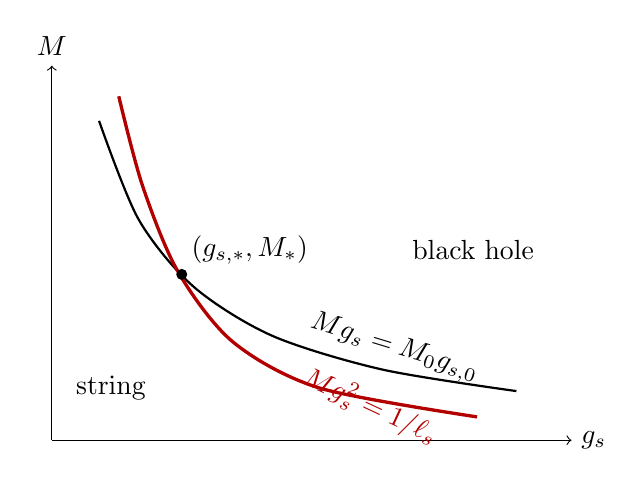
\begin{tikzpicture}[x=1cm,y=0.78cm]
  \draw[->] (0.4,0.4)--(7.0,0.4) node[right] {\(g_s\)};
  \draw[->] (0.4,0.4)--(0.4,6.5) node[above] {\(M\)};
  \draw[thick,black] plot[smooth] coordinates {(1.0,5.6) (1.5,4.0) (2.2,2.9) (3.2,2.1) (4.6,1.55) (6.3,1.2)};
  \draw[very thick,red!70!black] plot[smooth] coordinates {(1.25,6.0) (1.55,4.55) (2.0,3.15) (2.7,2.0) (3.8,1.25) (5.8,0.78)};
  \fill (2.05,3.1) circle (2pt) node[above right] {\((g_{s,*},M_*)\)};
  \node[black,rotate=-17] at (4.75,1.9) {\(Mg_s=M_0g_{s,0}\)};
  \node[red!70!black,rotate=-25] at (4.45,0.95) {\(Mg_s^2=1/\ell_s\)};
  \node at (5.75,3.5) {black hole};
  \node at (1.15,1.25) {string};
\end{tikzpicture}
\caption{黑板上的曲線圖及整理後的說明。黑色等熵曲線與較陡的紅色對應曲線相交；交點對應物體轉為弦態之處。}
\lectureframe{00:49:35.000}
\end{figure}

在交點 \((M_*,g_{s,*})\)，兩個方程式為
\begin{align}
M_*g_{s,*} &= M_0g_{s,0}, \\
M_*g_{s,*}^2 &\sim \frac{1}{\ell_s}.
\end{align}
將第一式平方，再除以第二式：
\begin{equation}
M_*
\sim M_0^2g_{s,0}^2\ell_s.
\end{equation}
接著乘以 \(\ell_s\)，得到
\begin{equation}
M_*\ell_s
\sim M_0^2g_{s,0}^2\ell_s^2
\sim M_0^2G_{N,0}.
\label{eq:l07-crossover-result}
\end{equation}

\begin{figure}[htbp]
\centering
\includegraphics[width=0.68\textwidth]{lecture_07_figure_08.png}
\caption{完整的過渡計算，包括 \(M_*\ell_s=M_0^2g_{s,0}^2\ell_s^2=M_0^2G_{N,0}\)。}
\lectureframe{00:54:40.000}
\end{figure}

\begin{classroomqa}
\audiencequestion{兩條曲線的方程式相除後，\(\ell_s\)應該在分子還是分母？\lecturetimestamp{00:52:41}}
\lecturerresponse{在分子。除以 \(1/\ell_s\) 等於乘以 \(\ell_s\)，所以 \(M_*\sim M_0^2g_{s,0}^2\ell_s\)。}
\end{classroomqa}

在過渡點上，弦熵公式適用，因此
\begin{equation}
S_*\sim M_*\ell_s.
\end{equation}
熵沿著路徑保持不變。結合這一點與方程式~\eqref{eq:l07-crossover-result}，便得到原先目標黑洞的熵：
\begin{equation}
S_{\mathrm{BH}}(M_0)
\sim M_0^2G_{N,0}
\sim M_0^2\ell_{p,0}^2.
\label{eq:l07-final-correspondence}
\end{equation}
這就是所要得到的面積律標度關係。

\section{對應關係論證的意義與限制}

這個論證並未宣稱原本的強引力黑洞就是自由弦。它先把物體帶到弦計數可靠的區域，在那裡求出熵，再沿可逆路徑將熵帶回原處。這是平滑的轉換過程，沒有明確的相邊界，因此這項估計無法決定方程式~\eqref{eq:l07-bh-exact}中的精確係數 \(1/4\)。

儘管如此，同樣的邏輯在標度上也適用於帶電黑洞、其他維度中的黑洞，以及延展的黑膜。對稱性較高、具有超對稱性的例子，則可以利用受保護的態計數，在耦合改變時保留精確資訊。這些方法能求出數值係數，但需要本講的概念性論證用不到的額外數學工具。

最重要的是，這項計算提供了微觀解釋。熵揭示了隱藏結構的存在。流體力學描述密度、壓力與流動，卻不直接描述分子；流體的熵則顯示，這些微觀自由度確實存在。廣義相對論同樣描述視界，卻不呈現其中的微觀態。弦的計數表明，自洽的量子引力理論可以包含足夠多的態，解釋黑洞熵。

\begin{classroomqa}
\audiencequestion{如果結果是 \(S\sim M^3\ell_p^3\)，而不是平方關係，會代表什麼？\lecturetimestamp{00:59:41}}
\lecturerresponse{那會是體積律。房間裡的普通物質或一杯咖啡，其熵正比於體積；平方關係之所以特殊，是因為透過 \(R_s\sim M\ell_p^2\)，熵正比於視界面積。}
\end{classroomqa}

這項結果顯示，貝肯斯坦--霍金熵不只是形式上的熱力學類比。它指向微觀的引力自由度，儘管基本推導並未逐一呈現這些自由度。

\section{從最大熵到全息原理}

現在我們換個問題：不再問指定狀態的熵是多少，而是問一個區域所能容許的最大熵是多少。

先從房間的普通格點模型開始。把體積分成大小為 \(V_{\mathrm{cell}}\) 的格子，每個格子都有一個二選一的問題：有物體占據，還是空著？Susskind刻意把想像中的原子取名為``meatonium''，這個荒唐的名稱可避免現實原子的細節干擾計數。若
\begin{equation}
N=\frac{V}{V_{\mathrm{cell}}},
\end{equation}
則組態數與最大熵為
\begin{equation}
\Omega=2^N,
\qquad
S_{\max}=\log\Omega=N\log2
\sim\frac{V}{V_{\mathrm{cell}}}.
\label{eq:l07-volume-count}
\end{equation}

\begin{figure}[htbp]
\centering
\includegraphics[width=0.68\textwidth]{lecture_07_figure_09.png}
\caption{房間分成許多格子，每格有兩種狀態。這裡計算的是最大熵，而非教室裡秩序井然的狀態所具有的熵。}
\lectureframe{01:05:20.000}
\end{figure}

實際房間的熵遠低於這個最大值。若一個狀態混亂地探索所有格子的可能狀態，溫度會高得驚人。這個簡化模型保留了普通的預期：獨立自由度的數目，以及因此而來的最大熵，會隨體積增加。

引力推翻了這個預期。考慮一個球形區域，其邊界面積為 \(A\)、初始熵為 \(S_{\mathrm{i}}\)，質量 \(M\) 小於恰好能填滿該球的黑洞質量 \(M_{\mathrm{BH}}\)。如果 \(M\) 更大，黑洞視界就已經超出所選的邊界。

現在送入一個質量為 \(M_{\mathrm{BH}}-M\) 的殼層。殼層由什麼組成並不重要；本講提到的例子包括光、普通物質，甚至瑞士起司。讓它坍縮後，最終狀態會是一個視界恰好填滿該區域的黑洞，其熵為
\begin{equation}
S_{\mathrm{f}}=\frac{A}{4G_N}.
\end{equation}
第二定律要求
\begin{equation}
S_{\mathrm{i}}\le S_{\mathrm{f}}
=\frac{A}{4G_N}.
\label{eq:l07-holographic-bound}
\end{equation}

\begin{figure}[htbp]
\centering
\includegraphics[width=0.70\textwidth]{lecture_07_figure_10.png}

\vspace{0.5em}
\begin{tikzpicture}[scale=0.88]
  \draw[thick] (0,0) circle (1.35);
  \draw[very thick,red!70!black] (0,0) circle (2.05);
  \fill[gray!25] (0,0) circle (1.32);
  \node at (0,0) {\(M,S_{\mathrm{i}}\)};
  \draw[-{Latex[length=3mm]},thick,red!70!black] (3.5,0)--(2.15,0);
  \node[align=center,right] at (3.5,0) {incoming shell\\\(M_{\mathrm{BH}}-M\)};
  \node[below] at (0,-2.2) {final horizon area \(A\)};
\end{tikzpicture}
\caption{殼層的構造。送入足夠的額外質量，使黑洞的視界恰好填滿所選區域。}
\lectureframe{01:13:30.000}
\end{figure}

這種大小的黑洞是允許存在的狀態，而且會使不等式取等號，因此最大熵為
\begin{equation}
S_{\max}=\frac{A}{4G_N}.
\label{eq:l07-holographic-maximum}
\end{equation}
這就是以計數方式表述的全息原理：引力區域中獨立自由度的最大數目，隨邊界面積而變；每個普朗克面積約對應一個數量級為一的自由度，而不是依據內部普朗克體積的數目而變。\editorialnote{殼層論證假設該區域能以所述方式被包圍並使其坍縮。更一般的時空需要使用協變熵界，但這個球形論證呈現了本講所要說明的原理。}

兩種計數的差距極大。局域場論的直覺認為，不同內部位置的選擇應能彼此獨立地組合，因而產生體積律。引力則指出，這類選擇若多到一定程度，就會自行坍縮；黑洞提供了更大的可容許熵。因此，邊界計數並非對體積計數稍作修正，而是以不同方式組織希爾伯特空間。

\begin{classroomqa}
\audiencequestion{對於密度大致均勻、尺度極大的宇宙，情況會如何？\lecturetimestamp{01:15:48}}
\lecturerresponse{這個問題需要用宇宙學來處理，不能只靠靜態球形區域的構造。它引出下一個主題：愛因斯坦方程的膨脹解。}
\end{classroomqa}

\begin{classroomqa}
\audiencequestion{面積界與不確定性原理有關嗎？\lecturetimestamp{01:16:03}}
\lecturerresponse{本講沒有回答這個問題，而是接著轉向宇宙學。}
\end{classroomqa}

\section{膨脹的空間}

這裡不會從愛因斯坦方程推導宇宙學解，而是直接寫出解，再學習如何解讀。空間切片可以是正曲率且封閉、負曲率且呈雙曲形，也可以是平坦的。以下討論的是時間相依時空中的平坦歐幾里得空間切片。

\begin{classroomqa}
\audiencequestion{普通歐幾里得空間在時空中的對應物是什麼？\lecturetimestamp{01:19:37}}
\lecturerresponse{閔考斯基時空。這裡討論的宇宙具有平坦的空間切片，但並非閔考斯基時空，因為空間度規會隨時間改變。}
\end{classroomqa}

熟悉的氣球比喻，描述的是低一個維度的封閉膨脹曲面。Susskind回憶曾試著用一個畫了標記的大氣球示範；記號筆削弱了橡膠，氣球便真的砰地一聲爆開。這場意外也點出了比喻在概念上的缺陷：普通氣球膨脹時，橡膠分子彼此遠離，材料逐漸變薄，最後破裂。宇宙空間卻不會因膨脹而稀釋局部物理定律。若要保留這個比喻，就得想像不斷加入新的橡膠分子，讓每一小塊區域維持相同的局部性質。在平坦模型中，可以把氣球換成一大片均勻向外拉伸、同時持續補充材料的薄片。

在數學上，膨脹由度規描述：
\begin{equation}
\begin{aligned}
ds^2&=-dt^2+a(t)^2d\mathbf{x}^2,\\
d\mathbf{x}^2&=\delta_{ij}\,dx^i dx^j
=dx^2+dy^2+dz^2.
\end{aligned}
\label{eq:l07-frw-metric}
\end{equation}

\begin{figure}[htbp]
\centering
\includegraphics[width=0.72\textwidth]{lecture_07_figure_11.png}
\caption{黑板上寫下的平坦空間膨脹度規。}
\lectureframe{01:25:10.000}
\end{figure}

空間座標保持不變的點稱為共動點。若兩個共動點的座標間隔為 \(\Delta x\)，則它們在時刻 \(t\) 的固有距離為
\begin{equation}
D(t)=a(t)\Delta x.
\label{eq:l07-proper-distance}
\end{equation}
兩點的座標沒有移動，但它們之間依度規定義的距離會改變。在固定 \(\Delta x\) 的條件下微分，得到
\begin{equation}
V=\dot D=\dot a\,\Delta x
=\frac{\dot a}{a}D.
\end{equation}
定義哈勃參數為
\begin{equation}
H(t)=\frac{\dot a(t)}{a(t)}.
\label{eq:l07-hubble-parameter}
\end{equation}
於是
\begin{equation}
V=H(t)D,
\label{eq:l07-hubble-law}
\end{equation}
這就是固定宇宙時間下的哈勃定律。

\begin{figure}[htbp]
\centering
\includegraphics[width=0.68\textwidth]{lecture_07_figure_12.png}
\caption{黑板上的等時退行定律：\(V=D\,\dot a/a\)。}
\lectureframe{01:29:10.000}
\end{figure}

「``哈勃常數''」這個名稱可能造成誤解。一般而言，\(H(t)\)會隨時間改變。同一時間切片上，任意一對共動點的比值 \(V/D\) 才是在空間中保持不變的量。

\begin{classroomqa}
\audiencequestion{對遙遠星系而言，這個關係中所用的是哪個時刻？我們觀測到的，是它們在較早時期的樣貌。\lecturetimestamp{01:31:10}}
\lecturerresponse{方程式~\eqref{eq:l07-hubble-law}描述的是等時情況。觀測沿著指向過去的光線進行，因此看到遙遠星系在較早時刻的狀態。要將測得的紅移與距離聯繫起來，必須考慮完整的光錐歷史，而不能只用 \(H\) 的某個瞬時值。}
\end{classroomqa}

\begin{figure}[htbp]
\centering
\includegraphics[width=0.66\textwidth]{lecture_07_figure_13.png}
\caption{時空示意圖，用以區分等時距離與觀測者沿指向過去的光線所觀察到的情況。}
\lectureframe{01:33:20.000}
\end{figure}

\section{哈勃尺度與德西特膨脹}

在 \(c=1\) 單位下，由方程式~\eqref{eq:l07-hubble-law}可知，在距離
\begin{equation}
D_H=\frac{1}{H}.
\label{eq:l07-hubble-radius}
\end{equation}
處，退行速度為一。更遠的共動點可以有 \(V>1\)，甚至 \(V\gg1\)，而不違反狹義相對論。它們並非以超光速掠過局部觀測者；它們之間的固有距離增加，是因為中間的空間幾何正在膨脹。\editorialnote{在一般的時間相依宇宙學中，\(1/H\)是哈勃半徑，但不一定是事件視界。在接下來討論的德西特情形中，它才是固定的視界尺度。}

在許多較早期的減速宇宙模型中，\(H(t)\)會減小，而 \(1/H(t)\)會增大，因此過去曾以超光速彼此遠離的區域，之後可能進入因果接觸。本講討論的晚期情況則趨近於一個正的常數 \(H\)。此時 \(1/H\)維持固定，膨脹方程式變為
\begin{equation}
\frac{\dot a}{a}=H,
\qquad
\dot a=Ha.
\label{eq:l07-constant-h}
\end{equation}

\begin{classroomqa}
\audiencequestion{固定的哈勃參數具有什麼單位？\lecturetimestamp{01:38:24}}
\lecturerresponse{時間的倒數。若取 \(c=1\)，也等同於長度的倒數。\(H^{-1}\)同時提供膨脹時間尺度與距離尺度；本講以約一百五十億年作為數量級的例子。}
\end{classroomqa}

方程式~\eqref{eq:l07-constant-h}的解為
\begin{equation}
a(t)=a_0e^{Ht}.
\label{eq:l07-desitter-scale-factor}
\end{equation}

\begin{classroomqa}
\audiencequestion{什麼函數的變化率與函數本身成正比？\lecturetimestamp{01:39:04}}
\lecturerresponse{指數函數。因此，尺度因子是 \(a_0e^{Ht}\)，而度規中的空間係數 \(a(t)^2\)則按 \(e^{2Ht}\) 增長。}
\end{classroomqa}

\begin{figure}[htbp]
\centering
\includegraphics[width=0.70\textwidth]{lecture_07_figure_14.png}
\caption{常數 \(H\) 情況下的方程式及其指數解，見黑板所示。}
\lectureframe{01:39:30.000}
\end{figure}

具有這種指數膨脹的時空稱為德西特空間。固定的哈勃尺度會在有限固有距離處形成事件視界。從某個角度看，這種幾何與黑洞圖像互為補充：觀測者留在宇宙學視界之內，足夠遙遠的物體則持續遠離，永遠無法發出訊號追上觀測者。黑洞視界對外部觀測者遮蔽內部；德西特視界則遮蔽觀測者可及區域之外的部分。與一般會蒸發的黑洞不同，這裡假設理想的德西特幾何持續存在。本講才剛開始比較這兩種情形；下一講將深入討論德西特視界、其熱力學，以及它為宇宙學帶來的難題。